\documentclass[tikz,border=2pt]{standalone}
\usepackage{amsmath,amssymb}
\usepackage{tikz}
\usetikzlibrary{arrows.meta}

\begin{document}
% A linear operator maps a space to itself: here the rotation of R^2 by 30 degrees, drawn in
% one and the same plane.
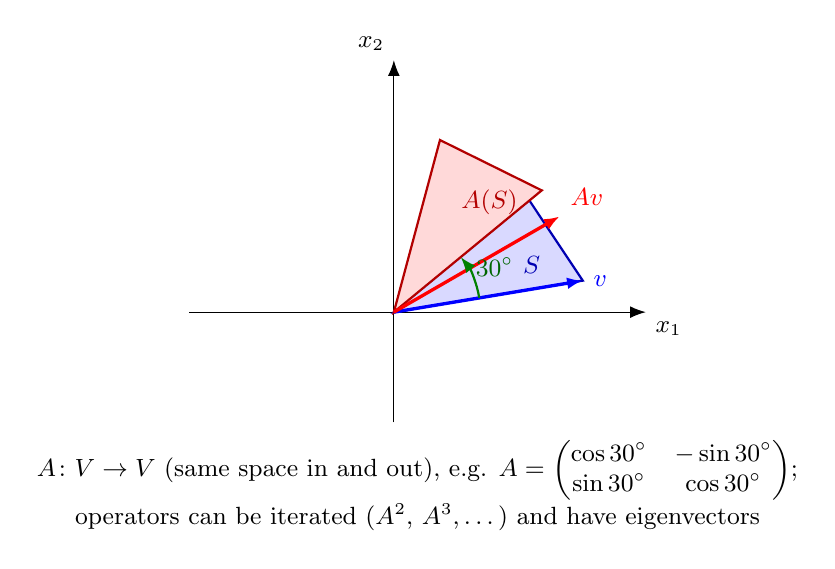
\begin{tikzpicture}[every node/.style={font=\small}, >={Latex[length=2mm]}]
	\draw[->] (-2.6,0) -- (3.2,0) node[below right] {$x_1$};
	\draw[->] (0,-1.4) -- (0,3.2) node[above left] {$x_2$};
	\fill[blue!15] (0,0) -- (2.4,0.4) -- (1.6,1.6) -- cycle;
	\draw[blue!70!black, thick] (0,0) -- (2.4,0.4) -- (1.6,1.6) -- cycle;
	\node[blue!70!black] at (1.75,0.6) {$S$};
	\begin{scope}[rotate=30]
		\fill[red!15] (0,0) -- (2.4,0.4) -- (1.6,1.6) -- cycle;
		\draw[red!70!black, thick] (0,0) -- (2.4,0.4) -- (1.6,1.6) -- cycle;
		\node[red!70!black] at (1.75,0.6) {$A(S)$};
	\end{scope}
	\draw[->, blue, very thick] (0,0) -- (2.4,0.4) node[right] {$v$};
	\draw[->, red, very thick] (0,0) -- (30:2.433) node[above right] {$Av$};
	\draw[green!50!black, thick, ->] (9.5:1.1) arc (9.5:39.5:1.1);
	\node[green!40!black, font=\small] at (24:1.4) {$30^\circ$};
	\node[anchor=north, align=center] at (0.3,-1.5) {$A\colon V\to V$ (same space in and out), e.g. $A=\begin{pmatrix}\cos30^\circ&-\sin30^\circ\\ \sin30^\circ&\cos30^\circ\end{pmatrix}$;\\ operators can be iterated ($A^2$, $A^3,\dots$) and have eigenvectors};
\end{tikzpicture}
\end{document}
